\documentclass[letterpaper]{article}
\usepackage{aaai16}

% Use the postscript times font!
\usepackage{times}
\usepackage{color}
\setlength{\pdfpagewidth}{8.5in}
\setlength{\pdfpageheight}{11in}

% the following package is optional:
\usepackage{latexsym}

\usepackage{graphicx}
\usepackage[centertags,fleqn]{amsmath}
\usepackage{amssymb,amsfonts,xspace}
\usepackage{booktabs}
\usepackage{theorem}
\usepackage{tikz}
\usetikzlibrary{arrows}
\usepackage{paralist}
\usepackage{enumitem}
\usepackage{centernot}
\usetikzlibrary{decorations.pathreplacing}
\usetikzlibrary{patterns}
\usetikzlibrary{positioning,chains,fit,shapes,calc}
\newcommand{\myproof}{\noindent {\bf Proof:\ \ }}
% \newcommand{}{\mbox{$\qed$}}
\newtheorem{mytheorem}{Theorem}
\newtheorem{question}{Question}
\newtheorem{myconjecture}{Conjecture}
\newtheorem{observation}{Observation}
\newtheorem{theorem}{Theorem}
\newtheorem{definition}{Definition}
\newtheorem{lemma}{Lemma}
\newtheorem{proposition}{Proposition}
\newtheorem{corollary}{Corollary}
\newtheorem{example}[theorem]{Example}
\newtheorem{conjecture}{Conjecture}
\newtheorem{fact}{Fact}
\newtheorem{remark}{Remark}
\newcommand{\qed}{\unskip\hspace*{1em}\hspace{\fill}$\Box$}
\newenvironment{proof}[1][Proof]{\begin{trivlist}
 \item[\hskip \labelsep {\it #1:}]}{%
 \qed\end{trivlist}}

	\usepackage[boxed]{algorithm}
	\usepackage[noend]{algorithmic}
	\renewcommand{\algorithmiccomment}[1]{\hfill\% #1}
	\renewcommand{\algorithmicrequire}{\textbf{Input:}}
	\renewcommand{\algorithmicensure}{\textbf{Output:}}
	\algsetup{linenodelimiter=\,}
	\algsetup{linenosize=\tiny}
	\algsetup{indent=2em}
	
	\newlength{\wordlength}
	\newcommand{\wordbox}[3][c]{\settowidth{\wordlength}{#3}\makebox[\wordlength][#1]{#2}}
 
%
% Paper Specific Macro's
%

%%% Notation Macros...
\newcommand{\clusterset}{\ensuremath{\mathcal{C}}}


% fix AAAI \cite command
\newcommand{\citen}[1]{\citeauthor{#1} \shortcite{#1}}
\newcommand{\citec}[1]{\citeauthor{#1} \citeyear{#1}}

%% SOME ABBREVIATIONS
\newcommand{\ie}{i.e.,\xspace}
\newcommand{\eg}{e.g.,\xspace}
\newcommand{\cf}{cf.\@\xspace}

	\newcommand{\midd}{\mathbin{:}}

	\newcommand{\pref}{R\xspace}
	%justified representation
\newcommand{\jr}{\ensuremath{\mathit{JR}}\xspace}
\newcommand{\ejr}{\ensuremath{\mathit{EJR}}\xspace}
\newcommand{\sjr}{\ensuremath{\mathit{SJR}}\xspace}


%\newcommand{\note}[1]{\textcolor{blue}{Note: #1}}
\newcommand{\note}[1]{}

\usepackage{mathtools}
\DeclarePairedDelimiter{\ceil}{\lceil}{\rceil}
\DeclarePairedDelimiter{\floor}{\lfloor}{\rfloor}
\DeclareMathOperator*{\argmin}{arg\,min}


\definecolor{kentuckyblue}{RGB}{0, 93, 170}			%Go Big Blue!
\definecolor{green}{RGB}{0, 102, 0}					%Haris Green
\definecolor{frenchred}{RGB}{250,60,50}				% French Red
\definecolor{unswyellow}{RGB}{255,155,0}			% Toby Yellow
\definecolor{purple}{RGB}{255,56,168}				%Mixing Canadian Red with Israeli Blue

\newcommand{\nick}[1]{\textcolor{kentuckyblue}{\textbf{Nick Says: #1}}}
\newcommand{\haris}[1]{\textcolor{green}{\textbf{Haris Says: #1}}}
\newcommand{\toby}[1]{\textcolor{unswyellow}{\textbf{Toby Says: #1}}}
\newcommand{\rupert}[1]{\textcolor{frenchred}{\textbf{Simon Says: #1}}}
\newcommand{\omer}[1]{\textcolor{purple}{\textbf{Omer Says: #1}}}



	% natbib workaround
	% Apt (2000)
	\newcommand{\citet}[1]{\citeauthor{#1}~\shortcite{#1}}
	% (Apt 2000)
	\newcommand{\citep}{\cite}
	% Apt 2000
	\newcommand{\citealp}[1]{\citeauthor{#1}~\citeyear{#1}}

% \nocopyright

\setlength\titlebox{2.20in}
\setcounter{secnumdepth}{2}


%  \pdfinfo{
%  /Title (Strategyproof Peer Selection: Mechanisms, Analyses, and Experiments)
%  /Author (Haris Aziz, Omer Lev, Nicholas Mattei, Jeffrey S. Rosenschein, Toby Walsh)
%  /Keywords (Computational Social Choice, Peer Selection, Mechanism Design)
%   }

\frenchspacing

\begin{document}
\title{Strategyproof Peer Selection: Mechanisms, Analyses, and Experiments}

\author{
Haris Aziz\\
Data61 and UNSW\\
Sydney, Australia\\
haris.aziz@nicta.com.au
\And
Omer Lev\\
University of Toronto\\
Toronto, Canada\\
omerl@cs.toronto.edu
\And
Nicholas Mattei\\
Data61 and UNSW\\
Sydney, Australia\\
nicholas.mattei@nicta.com.au
\AND
Jeffrey S. Rosenschein\\
The Hebrew University of Jerusalem\\
Jerusalem, Israel\\
jeff@cs.huji.ac.il
\And
Toby Walsh\\
Data61 and UNSW\\
Sydney, Australia\\
toby.walsh@nicta.com.au
}




\maketitle

\begin{abstract}
We study an important crowdsourcing setting where agents evaluate one another and, based on these evaluations, a subset of agents are selected. This setting is ubiquitous when peer review is used for distributing awards in a team, allocating funding to scientists, and selecting publications for conferences. The fundamental challenge when applying crowdsourcing in these settings is that agents may misreport their reviews of others to increase their chances of being selected. We propose a new strategyproof (impartial) mechanism called Dollar Partition that satisfies desirable axiomatic properties. We then show, using a detailed experiment with parameter values derived from target real world domains, that our mechanism performs better on average, and in the worst case, than other strategyproof mechanisms in the literature.	
\end{abstract}

\section{Introduction}
% The problem arising from letting people who are participating in a contest to rate the other contestants -- the \emph{peer selection problem} -- has been well known for millennia: people might report untruthfully on others in order to improve their own chances of selection.
 % The problem arising from letting people who are participating in a contest to rate the other contestants has been well known for millennia: people might report untruthfully on others in order to improve their own chances of selection.
 
The problem arising from using peer review to select contestants has been well known for millennia:
people might report untruthful valuations of others in order to improve their own chances of selection.
The problem has been referred to as the \emph{peer selection problem}.
Various techniques have been attempted to solve it, most of which focused on reducing the influence of other participants on the selection of winners, for example, by using lotteries to either replace selection or to be a heavy part of the process \cite{MG07}, 
%\haris{I wasn't sure what it means by ``using lottery to replace selection''. Are we not doing selection in any case?}\omer{I mean that they just randomly pick winners from some subset of candidates. Should a different phrase be used?}
or by using disinterested panels to prevent the participants of the contest from any influence at all.

Despite these measures, various settings in which each participant is both a candidate and a voter persist, for example, in the academic review process, various funding settings (the National Science Foundation (NSF) in the US is seeking to apply it to its funding allocation \cite{Haze13a}), and award decisions. Moreover, as the use of crowdsourcing in the online world is growing---from grading tasks in MOOCs to evaluating code in TopCoder \cite{LGE10}---the need for desirable peer selection mechanisms becomes more and more important. All these settings can be captured by a simple model: agents rate or rank one another (or some subset of their peers), and based on these reports a specified number of agents are selected. This problem has received much recent attention \citep{AFPT11a,FeKl14a,HoMo13a,KLMP15b,RRS11a}. Since peer review can be costly in terms of time and effort, each agent may be asked to review only a subset of other agents~\citep{KLMP15b,MeSa09a}.


The main challenge in the peer selection problem is to propose strategyproof (also called impartial) mechanisms in which agents cannot increase their chances of being selected by misreporting.\footnote{A strict incentive to report truthfully is not possible in strategyproof mechanisms, so strictly better mechanisms are impossible.} 
Natural approaches to solve the peer selection problem, such the application of a voting rule, are \emph{not} strategyproof (also called manipulable).
%including the straightforward use of voting procedures like Borda (we call this technique Vanilla).
%One approach to solve the peer selection problem is to simply apply a voting rule to it (. 
%However, such an approach has a crucial drawback: in all such mechanisms agents are incentivized to game the system and report strategically to increase their chance of being selected or of having a higher rank, according to the Gibbard-Satterthwaite theorem \cite{Gib73,Sat75}. %A typical strategy, which works in many cases, is to report a lower ranking to agents who are just ahead of the reporting agent in the aggregate ranking.
A different approach to the selection problem is to use mechanisms similar to the Page Rank algorithm that use Markov chains to compute a ranking of the agents \cite{Wals14a}. Unfortunately, these approaches are also manipulable. If a mechanism is manipulable, the normative properties of the mechanism (that hold under the assumption that agents do not misreport) may not hold in general. Hence, we primarily focus on strategyproof mechanisms, although we also consider some natural manipulable mechanisms as well to provide a ``best case'' comparison. 


 %and is related to that of \emph{ranking systems} in which agents vote over each other.

% and their votes are aggregated to obtain an overall ranking~\citep{AlTe05b,AlTe07a,AlTe08a,AlTe10a} (and, to some extent, also to work in distributed computing on leader election~\citep{FeKl14a}). One variant of this problem is when agents nominate a subset of agents, without ranking, and this particular setting has been termed as the \emph{prize nomination problem}~\citep{HoMo13a}.\omer{I wonder if this paragraph contains to many citations, and we should simply relegate them to the previous work section}



% or trying to ignore the cardinal values given to agents, but only the ordinal information given by each participant \cite{JoRa15a}. Unfortunately, these approaches are manipulable as well.

%In view of this challenge, we try to identify desirable \emph{impartial} mechanisms for the selection problem, in which no agent may gain by reporting untruthfully. Note that no better result can be achieved: making it \emph{worthwhile} for an agent to be truthful would mean its ranking of others influence its own outcome, destroying impartiality. Of course, it is impartial to randomly select $k$ agents (or to select the most preferred $k$ agents of one particular agent), but as we wish to select ``quality'' winners, we want to incorporate the views of all the agents. 


Strategyproofness can be trivially satisfied by randomly selecting $k$ agents or selecting the best $k$ agents according to one particular agent (as do dictatorship mechanisms in social choice), but as we wish to select ``quality'' winners, we want to incorporate the views of all the agents. 
An established way to achieve strategyproofness is to partition the agents into a set of clusters and then select a specified number of agents from each cluster based on the reports of agents \emph{outside} the cluster~\citep{AFPT11a}. We combine this partitioning principle with ideas from a fair division rule to divide a dollar (Dollar for short)~\citep{CMT08a}, to create a novel mechanism called \textbf{Dollar Partition}.

\smallskip
\textbf{Contributions:}\;
We provide a comprehensive survey and study of existing peer selection mechanisms.
We show that iteratively using a strategyproof mechanism for $k=1$ to select more than one agent is \emph{not} strategyproof. We conduct a detailed experimental comparison with previously introduced strategyproof mechanisms with regard to their ability to recover the ``ground truth''. This is the first experimental comparison of the performance of strategyproof peer selection mechanisms.

Our main contribution is a novel peer selection mechanism (Dollar Partition) that satisfies desirable axiomatic properties including strategyproofness and natural monotonicity properties. We prove that although Dollar Partition relies on the Dollar mechanism to share a bonus~\citep{CMT08a}, three natural peer selection mechanisms inspired from Dollar are manipulable. Dollar Partition has a number of advantages over previously introduced strategyproof mechanisms including the Partition mechanism and the Credible Subset mechanism~\citep{KLMP15b}. Dollar Partition returns better quality outcomes ex post than Partition if one cluster has most of the top-ranked candidates. In contrast to Credible Subset, Dollar Partition never returns an empty set.

Experimentally, Dollar Partition selects more agents from a higher grade more often, selects more agents from higher grades in the worst case, and does so more consistently, than any other strategyproof mechanism in the literature. In the worst case we found that Dollar Partition provides a $\geq 17\%$ improvement over the agents selected by Partition. Additionally, as the proportion of reviews per agent increases, Dollar Partition performs increasingly better than Partition, Credible Subset, and the other Dollar adaptations.



%
%\paragraph{Contributions}
%\begin{itemize}
%	\item We highlight some shortcomings of the standard partition strategyproof mechanisms. In particular, standard partition mechanisms in which a set number of agents are selected from each cluster can do badly ex-post if the clusters have lopsided balance of good agents in one of the clusters. Straightforward fixes of this problem lead to computational intractability and even lack of strategyproofity.
%	\item We then propose a new peer selection mechanism called Dollar Partition. It involves ideas from the `dividing the dollar mechanism' of \citet{CMT08a}, the `partition mechanisms' considered by \citet{HoMo13a} and \citet{AFPT11a}.%, and a natural rounding technique that ensures impartiality. 
%	%\item We show that apart from impartiality, Dollar Partition is impartial satisfies important monotonicity axioms. It also has advantages over the previous Partition mechanisms. We additionally suggest specific ways to implement Dollar Partition in view of some of the salient requirements that are present in real world peer review and fellowship nomination processes.
%		\item We then conduct a detailed experimental analysis of Dollar Partition and compare it with previously introduced impartial mechanisms in their ability to recover the `ground truth'. To the best of our knowledge, this is the first experimental comparison of the performance of impartial peer selection mechanisms. As the proportion of reviews per agent increases, Dollar Partition performs increasingly better than Partition and Credible Subset.

%\end{itemize}


\section{Related Work}

The criticism that prominent peer selection mechanisms such as ones under consideration by American and European funding bodies~\cite{MeSa09a,Haze13a} are \emph{not} strategyproof ~\citep{NaLi13a} has underscored the need to devise mechanisms with better incentive properties. The literature most directly relevant to this article is a series of papers on strategyproof (impartial) selection initiated by \citet{HoMo13a} and \citet{AFPT11a}. 
We overview these mechanisms in Section~\ref{mechSurvey}.
Most of the work on strategyproof peer selection focuses on the setting in which agents simply approve (nominate) a subset of agents~\citep{AFPT11a,BNV14a,FeKl14a,HoMo13a} with the latter three restricting attention to the setting in which exactly one agent is selected ($k=1$).
\citet{Mack15a} and \citet{BeGj14a} focused on axiomatic aspects of peer selection. \citet{KLMP15b} presented an interesting strategyproof mechanism (Credible Subset) that performs well when each agent reviews a few other agents.
%. \citet{HoMo13a}, \citet{FeKl14a}, and \citet{BNV14a} additionally consider the setting in which exactly one agent is selected ($k=1$).

% Both \citet{AFPT11a} and \citet{HoMo13a} examined the selection problem in which agents simply approve (nominate) a subset of agents. \citet{HoMo13a}, \citet{FeKl14a}, and \citet{BNV14a}  restrict their attention to setting in which exactly one agent is selected ($k=1$).
% \citet{FeKl14a} also presented a new ``permutation'' mechanism which achieves the same bound as the Partition mechanisms for $k=1$.
%\citet{AFPT11a} and \citet{HoMo13a} showed that for the peer selection problem, deterministic impartial mechanisms are extremely limited, and must sometimes select an agent with zero nominations even though agents are being nominated, or an agent with one nomination when another agent receives $n-1$ nominations~\citep{FeKl14a}. %\citet{AFPT11a} presented an impartial mechanism for the peer selection problem where agents are partitioned into equal sized clusters and roughly equal number of agents are selected from each cluster.
% In recent work inspired by \citet{AFPT11a}, \citet{FeKl14a} and \citet{BNV14a} considered the setting in which agents nominate some other agents and one agent is selected. 
%\citet{FeKl14a} improved on the analysis of the partition mechanism of \citet{AFPT11a}. They also presented a new ``permutation'' mechanism which achieves the same bound as the Partition mechanisms when $k=1$. \citet{BNV14a} further analyzed the Permutation mechanism of \citet{AFPT11a}. % and presented the slicing mechanism that performs well when the maximum number of votes of the most popular agent is high enough.
%\citet{KLMP15b} presented a more general mechanism called Credible Subset that is strategyproof but may select \emph{no winners} with non-zero probability. Credible Subset performs well when each agent reviews a few other agents, and this number is considerably smaller than $k$. %Our work is closely related to ranking systems in which agents rank each other~\citep{AlTe05b,AlTe07a,AlTe08a}.




%Recently, \citet{KLMP15b} presented a mechanism called Credible Subset that is impartial but may return no selection with non-zero probability. Credible Subset performs well when each agent reviews a few other agents, and this number is considerably less than than $k$. The mechanism we present is suitable when each agent reviews every other agents and also works when each agent review a few other agents. In this case, the agents that he does not review are considered to get zero score from the agent.

 %The mechanism we present is suitable when each agent reviews every other agents and also works when each agent review a few other agents. In this case, the agents that he does not review are considered to get zero score from the agent. 



%This area of peer selection has received increasing amounts of attention after the NSF decided to consider it as a mechanism for performing reviews in the Astronomy directorate \cite{MeSa09a,Haze13a}. This mechanism has not been without its critics for its demonstrate able lack of impartiality both theoretically and empirically \cite{NaLi13a,KLMP15a}.

%A slightly different family of mechanisms are those which deal with appropriate division of a shared resource. \citet{CMT08a} proposed an impartial mechanism to share a dollar. The mechanism is not impartial if one simply selects the $k$ agents with the maximum dollars shares. Our work is also related to ranking systems in which agents rank each other~\citep{AlTe05b,AlTe07a,AlTe08a}

%A slightly different family of mechanisms are those which deal with appropriate division of a shared resource. 

%\citet{CMT08a} proposed a strategyproof mechanism not for the peer selection problem (picking discrete items) but for the problem of sharing a dollar (dividing a continuous resource). For $k=1$, the mechanism can be used as peer selection randomized mechanism (which we refer to as Dollar Raffle) if the Dollar shares are used as probabilities of selection~\citep{FeKl14a}.


 %Another way to use the mechanism is iteratively, selecting agents by probabilities equal to the dollar share of the agents. This method that we refer to as DollartRaffle does consistently worse than Dollar Partition, which will be presented below. 

%\citet{CMT08a} proposed an impartial mechanism to share a dollar. The mechanism is not impartial if one simply selects the $k$ agents with the maximum dollars shares. \citet{Wals14a} presented a mechanism based on the Markov chains (similar to the Page Rank algorithm) for the agents to grade each other. Although the mechanism can be used to select $k$ agents with the highest weight, the mechanism is not impartial. Our work is also related to ranking systems in which agents rank each other~\citep{AlTe05b,AlTe07a,AlTe08a}

% \citep{AlTe05b,AlTe07a,AlTe08a,AlTe10a} presented a number of results on ranking systems where they characterized the Page Rank ranking system in terms of axioms and they showed which axioms of ranking systems are compatible or not compatible.


%,RaJo14a
The peer selection problem is also related to peer-based grading/marking~\citep{DeSh13a,JoRa15a,KWLC13a,PHCD+13a,Robi01a,Wals14a,WTL15a} especially when students are graded
based on percentile scores.
% The peer selection problem is also related to peer-based grading/marking~\citep{Robi01a}.
% Many in the MOOC community are interested in mechanisms to scale up
% peer marking, and a number of mechanisms have been proposed~\cite{DeSh13a,RaJo14a,JoRa15a,KWLC13a,PHCD+13a,Wals14a,WTL15a}. The peer selection problem is applicable to this domain when students are graded
% based on percentile scores.
% on a curve, i.e., grades are assigned according to a predetermined distribution (e.g., average/median are fixed, etc.). 
%In this case, students may benefit from marking others untruthfully, and if students engage in collusion, they may report higher valuations so everyone passes. Correcting for these biases has been the study of many works in this area the above referenced and \cite{RRS11a,Bout12a}.
%especially if the grades are based on percentiles.
% The peer grading involves different incentives issues such as strictly incentivising disinterested or lazy students to give accurate peer grades.
For peer grading, mechanisms have been proposed that make a student's grade slightly dependent on the student's grading accuracy (see e.g., \citet{Wals14a} and \citet{MeSa09a}). However such mechanisms are not strategyproof since one may alter one's reviews to obtain a better personal grade.


%A different mechanism, although not an impartial one, was suggested in \citet{Wals14a}, which presented a mechanism based on the Markov chains (similar to the Page Rank algorithm) for the agents to grade each other. 
%\citet{JoRa15a} has proposed another impartial mechanism in which a ranking is created by ignoring the cardinal values assigned by participants, and only taking into account the ordinal ranking between the candidates graded by each participant, aggregating the grades to maximize a posterior distribution.\haris{Is the mechanism of Jora15a really impartial?}




%\nick{To Add: Discussion of grading on a curve, we need that students are competing for this to be necessary.}\omer{Added some. Think something larger is needed?}






\section{Setup and Survey of Existing Mechanisms}\label{mechSurvey}

%\subsection{Setup}

We have a set $N$ of agents $\{1,\ldots, n\}$. Each agent reports a valuation over the other agents. These messages could be cardinal valuations $v_i(j)$ for agent $i$'s valuations of agent $j$, or they could be a weak order reported by agent $i$ of agents in $N\setminus \{i\}$, which may be transformed to cardinal valuations using some predetermined scoring rule. 
An agent, depending on the setting, evaluates some $0 \leq m \leq n-1$ of the other agents.
Based on these messages, around $k$ agents are selected.
Some mechanisms such as Credible Subset and Dollar Partition may not always return a size of exactly $k$ even if the \emph{target} size is $k$.


%We give an overview of different mechanisms.

The general idea of the partitioning based mechanisms is to divide the agents into a set of clusters $\clusterset = \{C_1, \ldots C_{\ell}\}$. This clustering can be done using a random process or by a predetermined order, without adding randomness to the process. We will often abuse notation and refer to the value that one cluster has for another cluster $v_{C_i}(C_j)$; the valuation of all agents in $C_i$ for the agents in $C_j$: $\sum_{r \in C_i, j \in C_j} v_r(j)$.
% By this we mean the normalized sum of the valuation of all agents in $C_i$ for the agents in $C_j$, $\sum_{r \in C_i, j \in C_j} \frac{v_r(j)}{\sum_{k \in \{N \setminus C_i\}} v_r(k)}$.
%By this we mean the sum of the valuation of all agents in $C_i$ for the agents in $C_j$: $\sum_{r \in C_i, j \in C_j} v_r(j)$. 

\subsection{Mechanisms}

We outline some prominent peer selection mechanisms.

\begin{itemize}[leftmargin=*]
	 \setlength\itemsep{0em}
	% \item \emph{Balanced} Partition: Find a balanced partition and then implement the partition mechanism. In general, any reasonable notion of balanced will work. We will specifically use the minimal margin to define balanced but note that Example \ref{ex:balanced-not-impartial} holds for any specific notion of balanced based cutoffs. Define the margin between two clusters $i,j$ as $| v_{C_i}(C_j) - v_{C_j}(C_i) |$. By minimizing the sum of margins over all pairs of clusters in our clustering we have a balanced clustering where each of the clusters have roughly the same score. We say a clustering is \emph{perfectly balanced} if the sum of all the margins between all pairs of clusters is 0. The balanced partition mechanism chooses a clustering which minimizes the margin. If more than one clustering has minimal margin, we assume we select amongst these clusterings at random.
	
%\item 	Partition: Divide the agents into $\ell$ clusters. From each cluster choose a fixed number of agents based on the valuations of agents outside the cluster.
%	\item \textbf{Partition}: Divide the agents into ${\ell}$ clusters. From each cluster a preset number of agent are selected by the agents \emph{not} in that cluster. This class of mechanisms, is a straightforward generalization of the Partition mechanism studied by \citet{AFPT11a} (and in an early version of \citet{KLMP15b}).

\item \textbf{Vanilla}: %Each agent reviews $m$ other agents. 
select the $k$ agents with highest total value based on their reviews by other agents.
%Based on values that agents receive in their reviews, the $k$ agents with the highest total values are selected. 
Vanilla is not strategyproof; unselected agents have an incentive to lower the reported valuations of selected agents. 
\item \textbf{Partition}: divide the agents into ${\ell}$ clusters. and select a preset number of agents from each cluster, typically $k/\ell$, according to the valuations of the agents \emph{not} in that cluster. This class of mechanisms is a straightforward generalization of the Partition mechanism studied by \citet{AFPT11a} (and in an early version of \citet{KLMP15b}) and is strategyproof. 
\item \textbf{Credible Subset}~\citep{KLMP15b}: 
%Each agent reviews $m$ other agents; and $k$ out of a total of $n$ agents are selected. 
let $T$ be the set of agents who have the top $k$ scores. 
Let $P$ be the set of agents who do not have the top $k$ scores but will make it to the top $k$ if they do not contribute any score to all other agents. 
With probability $(k+|P|)/(k+m)$, Credible Subset selects a set of $k$ agents uniformly at random from $T\cup P$, and with probability $1-(k+|P|)/(k+m)$, it selects no one. The mechanism is strategyproof. %This only makes sense if $|P|\leq m$. \textbf{Omer can you please comment why $|P|\leq m$?}
%\item Random: choose $k$ at random.
%\item \textbf{Dollar Raffle}: compute the relative fractions of how much of a dollar each agent should get via the Dollar mechanism of \citet{CMT08a}. Using these shares as probabilities randomly select an agent according to its dollar share probabilities until $k$ different agents are selected. %(Note that this mechanism gives non-zero probability of selecting the worst $k$ agents and relies on a lot of randomisation).


%\item RandomDictator: choose agent uniformly at random and then select $k-1$ more agents who are the dictator's most preferred. (Note that this mechanism is not too bad if the peer evaluations are highly correlated but it gives a reasonable probability to select the unanimous worst agent).

%	\item \emph{MarkovPartition} mechanism: 
	%\item Dollar Partition mechanism:
\end{itemize}
% The general idea of the last two mechanisms is to partition the agents into ${\ell}$ clusters $C_1,\ldots, C_{\ell}$, then find the share $x_i$ of each cluster $C_i$ by Markov chain over the clusters or by `Dividing the Dollar' mechanism, make the shares integers by using some apportionment mechanism, and then use the Partition approach to select the required number of agents from each cluster.


% \begin{remark}
% 	A randomized mechanism for $k=1$ can be adapted for general $k$ can be adapted as follows: keep rerunning the mechanism until $k$ different outcomes are produced. Question is whether impartiality is lost or maintained after doing this.
% 	\end{remark}


Some other mechanisms are tailor-made for $k=1$ and for the case where agents only approve a subset of agents: Partition by \citet{HoMo13a}; Permutation by~\citet{FeKl14a}; and Slicing by~\citet{BNV14a}.
We take inspiration from the Dollar mechanism designed to split a divisible resource \cite{CMT08a}.

%resource that is not a peer selection mechanism but a mechanism to divide a Dollar of bonus based on agents' opinion on how much other agents contributed. 

%\noindent\\

\begin{itemize}
\item \textbf{Dollar}: Each agent $i$ has a value $v_{i}(j)$ of his estimation of how much $j$ should get. We assume these values are normalized so that $\sum_{j\in N\setminus \{i\}}v_i(j)=1/n$. Then the \emph{Dollar share} of each agent $i$ is $x_i=\sum_{j\in N\setminus \{i\}}v_j(i)$.
\end{itemize}



%	\item \emph{PeerRank}: Each agent reports cardinal valuations. Based on the weighted tournament represented by the valuations, the stationary distribution of the Markov chain is computed which gives the relative scores of the agents. By selecting the agents with the top $k$ scores, one can use PeerRank as a nomination rule. 



%The mechanisms of \citet{HoMo13a} can be ignored because seem to crucially depends on the assumption that each agent approved exactly one agent. The mechanisms of \citep{FeKl14a} and \citep{BNV14a} are for $k=1$ but maybe this is not reason to dismiss them because for more general $k$, one can simply rerun the mechanism until $k$ different outcomes are produced. \textbf{Question is whether impartiality is lost or maintained after doing this.}


\subsection{Properties of Mechanisms}

We consider some basic axioms of peer selection mechanisms:
\begin{inparaenum}[(i)]
	% \item \emph{Unanimity}: If %cluster sizes are of size at least $2$ and
	% valuations are unanimous and $k=1$, the worst candidate will not be selected (this is true for Partition and Dollar Partition).
	\item \emph{Non-imposition}: for any target set $W$, there is a valuation profile and a randomization seed that achieves $W$;
	\item \emph{Strategyproofness (Impartiality)}: agents cannot affect their own selection;
	\item \emph{Monotonicity}: if an agent $i$ is selected, then if in a modified setting in which that agent is reinforced (score or ordinal ranking of $i$ is improved with respect to other agents) by some other agents and no other agent's value/ranking improved, then $i$ will remain selected;
	\item \emph{Committee Monotonicity}: if $W$ is the outcome when the target set size is $k$, then the agents in $W$ are still selected if the target set size is $k+1$. (The final two properties are in expectation when algorithms involve randomization.)
\end{inparaenum}

%Observation: if cluster sizes are of size at least $2$ and evaluation are unanimous and $k=1$, then any partition mechanism will not select the unanimous worst one. 

%May need formal definitions as well.\omer{I don't think they do. Will kill us with length...}
% \begin{itemize}
% %	\item If $k=n-1$, then the mechanism selects the best agent. (this axiom is not satisfied by permutation and also slicing I think. It is also not satisfied by credible sub)
% 	\item If %cluster sizes are of size at least $2$ and
% 	valuations are unanimous and $k=1$, the worst candidate will not be selected (this is true for Partition and Dollar Partition).
% %	\item If $k=n-1$, then the mechanism selects the best agent. (this axiom is not satisfied by permutation and also slicing I think. It is also not satisfied by credible subset). \omer{Think we should drop this: If the ``best'' is due to very few very heavy edges, then no partition mechanism satisfies this too.}
% 	\item \emph{Non-imposition}: For any target set $W$, there is a valuation/preference profile and a randomization seed that achieves $W$.
% 	\item \emph{Impartiality}: agents cannot affect their nomination.
% 	\item \emph{Monotonicity}: if an agent $i$ is selected, then if in a modified setting in which that agent is reinforced by some other agents, it will remain selected.
% 	\item \emph{Committee Monotonicity}: If $W$ is the $k$-sized set of agents selected, then these agents are still selected if $k$ is incremented by one.
% \end{itemize}

	
\section{Dollar Partition}

	

Dollar Partition is formally described as Algorithm~\ref{algo:DP}. The algorithm works as follows. First, agents are partitioned such that the difference between the sizes of any two clusters is at most one. Each agent $i\in N$ assigns a value $v_i(j)$ to each agent $j$ that is in a cluster other than $i$'s cluster and $j$ is among the $m$ agents that $i$ reviews. Agent $i$ may directly give a cardinal value to the agents he reviews or the cardinal value may be obtained by a scoring function that converts the ordinal ranking given by $i$ to cardinal values. In either case, the values that $i$ gives are normalized so that agent $i$ assigns a total value of 1 to agents outside his own cluster. Based on the values from agents outside the cluster, each cluster $C_j$ gets a normalized weight of $x_j$, its assigned share. Based on each share $x_i$, each cluster gets a quota $s_i=x_i \cdot k$ which may be a non-integer number.\footnote{After AAAI-2016 publication, we recognized our (required) implicit assumption that $k \leq n/\ell$.}
%or $s_i \geq |C_i|$. 
%\haris{We will assume that $k\leq n/\ell$.} %$\ell \geq n/k$.
	If all $s_i$'s are integers that are at most the size of the corresponding cluster, then each $s_i$ is the quota of cluster $C_i$, i.e., exactly $s_i$ agents are selected from cluster $C_i$. 
If not all $s_i$ are integers, we take the ceiling of each $s_i$ and use this as the quota for $C_i$.
Note that the size of the winning set may be larger than $k$: $|W| \leq k+\ell-1$.\footnote{In practical settings this may not be a problem, since often a couple of more winners can be accommodated (e.g., shortlists etc.\ in case of agents declining awards).}
%, or the award committee may have a shortlist that is slightly larger than the number of awardees, in case some agents decline the award.}  
%As long as $\ell$ is a small integer (usually $\approx 3$) and $k$ is reasonably large, $|W| \approx k$.
As long as $\ell$ is a small integer and $k$ is reasonably large then $|W| \approx k$.\footnote{One would think that if each cluster does not get an integer share, then one can consider various apportionment rules, which have been suggested in the literature in the past several centuries, in particular in political science~\cite{Youn94a}. However, applying these rules violates the strategyproofness of the overall mechanism.}
	
	
	
Note that if the partitioning into clusters and the review allocation can be done in a deterministic manner (e.g., lexicographic ordering), Dollar Partition is deterministic. We first prove that Dollar Partition is strategyproof.

% Note that Dollar Partitioning has two stages of randomization: firstly a partitioning is generated at random. Secondly, clusters are chosen according to probability distribution $x$ so that their quota is incremented by one.



		\begin{algorithm}[ht!]
		 \caption{Dollar Partition}
		 \label{algo:DP}
		\renewcommand{\algorithmicrequire}{\wordbox[l]{\textbf{Input}:}{\textbf{Output}:}} 
		 \renewcommand{\algorithmicensure}{\wordbox[l]{\textbf{Output}:}{\textbf{Output}:}}
		\algsetup{linenodelimiter=\,}
		%\small
		\footnotesize
		\begin{algorithmic}
			\footnotesize
			\REQUIRE $(N,v,k)$; the algorithm is parametrized by number of clusters $2\leq \ell\leq n$ and $m$, the number of reviews per agent.
			\ENSURE $W\subset N$ such that $|W|\leq k+\ell-1$
		\end{algorithmic}
		 \begin{algorithmic}[1] 
			% \normalfont
				%\small
				\footnotesize
		
			 \STATE Initialize $W\longleftarrow \emptyset$
			 \STATE Generate a partition $\{C_1,\ldots, C_{\ell}\}$ of $N$ in which the difference between the sizes of any two clusters is at most 1. Let $C(i)$ be the cluster of agent $i$. %\COMMENT{The partition could be generated randomly or could be deterministic by some preset order (e.g., according to registration order), with cluster cutoff for every $n/\ell$.}
%			 \COMMENT{For each $i\in N$, we denote by $C(i)$ the cluster of agent $i$. }
			 \STATE 
			 Each $i\in N$ reviews $m$ agents outside $C(i)$.
			 Ensure $v_i(j)=0$ for $j\in C(i)$ and that $\sum_{j\notin C(i)}v_i(j)=1$ by setting the valuation of agent $i$ for agents in its cluster to $0$ and normalizing.
			 %We will assume $v_i(j)=0$ for $j\in C(i)$ and that $\sum_{j\notin C(i)}v_i(j)=1$. 
			 %\COMMENT{If this is not the case we ignore the valuation of agent $i$ for agents in its cluster and normalize its valuations for agents outside it. %Hence each agent $i\in N$ gives a total value of one to agents in clusters other than $C(i)$.
			 %} 
			 %In case, agents express ordinal preferences, these ordinal preferences are converted to cardinal values via scoring rules such as Borda. 
			 	 
		 \STATE $x_i$ value of a cluster $C_i$ is defined as follows:
		% \vspace{-1em}
			 \[x_i\longleftarrow \frac{1}{n} \times \sum_{j\in C_i, j'\notin C_i}v_{j'}(j).\] 
			%  \vspace{-1em}
%			Hence, $\vec{x}=(x_1,\ldots, x_{\ell})$ is a probability distribution.% over clusters.
			%\COMMENT{Since $x_i$s sum up to one, the $\vec{x}=(x_1,\ldots, x_{\ell})$ can also be used as a probability distribution over the clusters}. 
			 \STATE Using the $x_i$ values, we compute the number of agents $t_i$ to be chosen from each cluster $C_i$. We first compute each $s_i$.
 \[s_i\longleftarrow x_i * k \text{ for each } i\in \{1,\ldots, \ell\}.\] 
% \[\vec{s}=(s_1,\ldots, s_{\ell}).\]
	
			
			% \IF{$s_i\in \{0,\ldots, |C_i|\}$ for all $i\in \{1,\ldots, m\}$}
			% \STATE $t_i \longleftarrow s_i$
			% 	\ELSIF{$s_i\notin \{0,\ldots, |C_i|\}$ for some $i\in \{1,\ldots, m\}$}
			 			 \FOR{each $i\in \{1,\ldots, \ell\}$}
			 			 \STATE $t_i \longleftarrow \min(\text{Ceiling}{(s_i)}, |C_i|)$.
%\footnote{Round can be the ceil function, floor function, or simply round up or down depending whether the fraction is more than 1/2 with ties broken arbitrarily. We opt for $Round=ceil$.}						 
					%	 \COMMENT{Round can be the ceil function, floor function, or simply round up or down depending whether the fraction is more than 1/2 with ties broken arbitrarily. We opt for $Round=ceil$.}
			 			 \ENDFOR
				% \ENDIF
				\STATE For each $i\in C(i)$, the score of agent $i$ is 
				 $\sum_{i'\notin C(i)}v_{i'}(i).$
				 \STATE Select $t_j$ agents with the highest scores from each cluster $C_j$ and place them in set $W$.
			\RETURN $W$		
		 \end{algorithmic}
		\end{algorithm}







 % 		\begin{algorithm}[h!]
 % 		 \caption{Dollar Partition}
 % 		 \label{algo:DP}
 % 		\renewcommand{\algorithmicrequire}{\wordbox[l]{\textbf{Input}:}{\textbf{Output}:}}
 % 		 \renewcommand{\algorithmicensure}{\wordbox[l]{\textbf{Output}:}{\textbf{Output}:}}
 % 		\algsetup{linenodelimiter=\,}
 % 		\begin{algorithmic}
 % 			\REQUIRE $(N,v,k)$; the algorithm is parametrized by number of clusters $2\leq \ell\leq n$.
 % 			\ENSURE $W\subset N$ such that $|W|=k$
 % 		\end{algorithmic}
 % 		 \begin{algorithmic}[1]
 % 			 \normalfont
 % 			 \STATE Initialize $W\longleftarrow \emptyset$
 % 			 \STATE Generate a partition $\{C_1,\ldots, C_{\ell}\}$ of $N$ in which the difference between the sizes of any two clusters is at most one. \COMMENT{The partition could be generated randomly or could be deterministic.}
 % 			 \STATE For each $i\in N$, we denote by $C(i)$ the cluster of agent $i$. We will assume $v_i(j)=0$ for $j\in C(i)$ and that $\sum_{j\notin C(i)}v_i(j)=1$. If this is not the case we can simply ignore the valuation of agent $i$ for agents in this cluster and normalize his valuations for agents outside his cluster. Hence each agent $i\in N$ gives a total value of one to agents in clusters other than $C(i)$.
 % 		 \STATE $x_i$ value of a cluster $C_i$ is defined as follows:
 % 			 \[x_i\longleftarrow (\sum_{j\in C_i, j'\notin C_i}v_{j'}(j))/n\]
 % 			 Since $x_i$'s sum up to one, the $x=(x_1,\ldots, x_{\ell})$ can also be used as a probability distribution over the clusters which we use later.
 % 			 \STATE Using the $x_i$ values, we compute the number of agents $t_i$ to be chosen from each cluster $C_i$. In order to compute each $t_i$, we first compute each $s_i$.
 % \[s_i\longleftarrow x_i * k \text{ for each } i\in \{1,\ldots, m\}.\]
 % \[\vec{s}=(s_1,\ldots, s_{\ell}).\]
 % 			 % \IF{$\sum_{i} \floor{s_i} = k$}
 % 			% \STATE $\vec{s}$ is finalized.
 %
 % 			\IF{$s_i\in \{0,\ldots, |C_i|\}$ for all $i\in \{1,\ldots, m\}$}
 % 			\STATE $t_i \longleftarrow s_i$
 % 				\ELSIF{$s_i\notin \{0,\ldots, |C_i|\}$ for some $i\in \{1,\ldots, m\}$}
 % 			 			 \FOR{each $i\in \{1,\ldots, m\}$}
 % 			 			 \STATE $t_i \longleftarrow \min(\floor{s_i}, |C_i|)$\label{smallDiff}
 % 			 			 \ENDFOR
 % 								\STATE $k'\longleftarrow \sum_{i} t_i$.
 % 								\WHILE{$k'\neq k$}
 % 				\STATE select a cluster $C_i$ with probability $x_i$;
 % 				\STATE $t_i\longleftarrow t_i+1$
 % 				\STATE $k'\longleftarrow k'+1$.
 % 				\ENDWHILE
 % 				\ENDIF
 % 				\STATE For each $i\in C(i)$, the score of agent $i$ is
 % 				 \[\sum_{i'\notin C(i)}v_{i'}(i).\]
 % 				 \STATE Select $t_j$ agents with the highest scores from each cluster $C_j$ and place them in set $W$.
 % 			\RETURN $W$
 % 		 \end{algorithmic}
 % 		\end{algorithm}
		
		% For the three possible versions of Round function specified in the algorithm, the size of the winning set $W$ is as follows: $k-\ell+1\leq |W| \leq k+\ell-1$. As long as $\ell$ is a small integer such as three and $k$ is reasonable large, the size of the winning set is roughly $k$. In particular, if we round up and down depending on whether the decimal number is above or below 0.5, then the expected winning set size is exactly $k$. Rounding up (taking the ceiling) will lead to a maximum of extra $\ell$ agents being selected
		
		
	
		% \begin{remark}
		% 	If we round up and we get $k+\ell-1$ agents, we can set the target size to be $k-1$ which will gives us at most $\ell$ less agents. We can keep decreasing untill the target winning set size is either $k$ or just above $k$. Does this work?
		% 	\end{remark}	
		


%
%
% \begin{enumerate}
% \item Let $s_i$ be the share of $i$ defined as $x_i * k$.
% \item If $\sum_{i} \floor{s_i} = k$ then return $\vec{s}$ Return...
% \item Foreach $i$: if $\lceil s_i \rceil - s_i > \frac{1}{n}$ then $s_i = \lfloor s_i \rfloor$ else $s_i = \lceil s_i \rceil$
% \item If $\sum_{i} s_i == k $ then Return...
% \item If $\sum_{i} s_i < k $ then increment $k - \sum_{i} s_i$ clusters according to the distribution induced by the dollar shares and increase shares of the selected clusters by 1 (with replacement).
% choose a cluster according to the $x_i$ probability distribution and increase their share by 1.
%
% \item Else $\sum_{i} s_i > k$ then select $\sum_{i} s_i - k$ according to the inverse dollar share distribution given by $\forall i: \frac{1 - x_i}{\sum_{j}1- x_i}$ and decrease shares of the selected clusters by 1 (with replacement).
% \end{enumerate}

\begin{theorem}
	Dollar Partition is strategyproof.
	\end{theorem}
	\begin{proof}
		Suppose agent $i$ is in cluster $C_j$ of the generated partition. Agent $i$ will be selected in $W$ if and only if its rank according to the $v$ scores given by agents outside of $C_j$ is at least $t_j$. Therefore agent $i$ can either manipulate by increasing $t_j$ or by increasing its score relative to other agents in $C_j$ given by agents outside $C_j$. Since agent $i$ cannot affect the latter, the only way it can manipulate is by increasing $t_j$. 
		We argue that agent $i$ cannot change $t_j$ by changing his valuation $v_i$ for agents outside the cluster. Note that $i$ contributes a probability weight of $1/n$ to agents outside $C_j$ and zero probability weight to agents in $C_j$. Hence it cannot affect the value $x_j$ of cluster $C_j$. As $s_j$ is derived from $x_j$, agent $i$ cannot affect the number $t_j= \min({\text{Ceiling}(s_j)},|C_j|)$.
%		Therefore $s_j=x_j * k$ is the fractional number of agents to be selected from $C_j$. In particular $\min({\text{Ceiling}(s_j)},|C_j|)$ is the number of agents to be selected from $C_j$.		
	\end{proof}
	
	Dollar Partition easily satisfies non-imposition; we show it satisfies other 
	key monotonicity properties.
%	Next, we prove that Dollar Partition satisfies desirability monotonicity properties.
	
	% \emph{Committee Monotonicity}: For a valuation profile $v$, the probability of $i$ being selected for $k+1$ is least as much as that of $i$ being selected for target winning set $k$.
	
		
		% \emph{Monotonicity}: For a valuation profile $v$, let us that $v'$ is exactly the same except that for some agent $j$ and some agents $k,i$ ($k\neq i$), $v_j'(k)=v_j(k)-\epsilon$ and $v_j'(i)=v_j(i)+\epsilon$. Then, the probability of $i$ being selected for valuation profile $v'$ is at least as much as that of $i$ being selected for valuation profile $v$.

		
		\begin{theorem}
			Dollar Partition is monotonic. 
			\end{theorem}
			\begin{proof}
				% NEED TO WRITE THE RIGHT DEFINITION OF MONOTONICITY SO THAT THE CLUSTER'S PROBABILITY DOES NOT DECREASE. For a valuation profile $v$, let us that $v'$ is exactly the same except that for some agent $j$, $v_j'(k)=v_j(k)-\epslion$ and $v_j'(i)=v_j(k)+\epslion$. Then
	
	%\nick{This is a bit messed up -- Haris is thinking about it.}
	Let us compare the valuation profile $v$ when $i$ is not reinforced and $v'$ when $i$ is reinforced. 
The relative ranking of $i$ is at least as high when $i$ is reinforced. Since any decrease in valuation that an agent $j$ in $C(i)$ receives translates into the same increase in the valuation received by agent $i$, hence the total valuation that $C(i)$ receives does not decrease and hence the number of agents to be selected from $C(i)$ is at least as high as before. 
		%
	% The share of $i$'s cluster of is at least as large for $v'$ as it was for $v$ (the same if changes were for agents in the same cluster. Strictly larger if they in different ones). Furthermore, the relative position of $i$ in its cluster is at least as good for $v'$ as for $v$. Hence, probability of $i$ being selected for valuation profile $v'$ is at least as much as that of $i$ being selected for valuation profile $v$.
\end{proof}

	\begin{theorem}
		Dollar Partition is committee monotonic. 
		\end{theorem}
		\begin{proof}
The only difference between running the algorithm for different target $k$ values is when calculating the share vector $\vec{s}$. However, if agent $i$ in cluster $C_{j}$ was selected, that means its ranking in the cluster $C_{j}$ was above $t_{j}=\min(\text{Ceiling}(s_{i}),|C_{j}|)$. When $k$ increases, $s_{i}$ will only increase (as $x_{i}$ remains the same), and hence so will $t_{j}$, ensuring that $i$ will be selected again.% I.e., in any partition in which $i$ was selected for a smaller $k$, it will be selected with a larger one.
			\end{proof}

%\begin{remark}


Although Dollar Partition draws inspiration from Dollar and Partition, it has key differences from these approaches.

%\paragraph{Comparison with other Dollar based mechanisms}
%
%Although Dollar Partition is partly based on the Dollar mechanism for dividing a bonus, it is more desirable than other natural impartial peer selection mechanisms based on the Dollar framework. Dollar Raffle relies too much on randomization and gives even the worst agents non-zero probability of being selected. 
%\haris{Dollar Raffle is strategyproof for $k=1$ but it is not clear that Dollar Raffle is strategyproof for $k>1$.} 
%
%We can also define another mechanism \textbf{Dollar Partition Raffle} to select exactly $k$ agents. This extension takes the dollar shares of the \emph{clusters} in Dollar Raffle and uses these shares to define a probability distribution over the partitions. When then select the top agents (that have not already been selected) from partitions until we have $k$ agents. %This extension remains strategyproof and selects exactly $k$ agents. 
%\haris{It is not clear that Dollar Partition Raffle is strategyproof.}
%
%Although Dollar Partition Raffle relies less on the ``luck of the draw'', it still admits non-zero probability of selecting the worst $k$ agents if the same cluster (consisting of the worst agents) is selected repeatedly. Dollar Partition Raffle is equivalent to Dollar Raffle if $\ell=n$.
%
%Another possible approach is that $k$ agents with the maximum dollars shares are selected. However such a mechanism is \emph{not} an strategyproof peer selection mechanism because an agent who is not selected may get selected by giving lower score to the agents who are selected.

\smallskip
\noindent
\textbf{Comparison with other Dollar Based Mechanisms:}\;
Although Dollar Partition is partly based on the Dollar mechanism for dividing a bonus, it is more desirable than other peer selection mechanisms based on the Dollar framework:
\begin{itemize}[leftmargin=*]
	\setlength\itemsep{0em}
\item \textbf{Dollar Raffle} computes the relative fractions of how much of a dollar each agent should get via the Dollar mechanism of \citet{CMT08a}. Using these shares as probabilities, do the following $k$ times: randomly select an agent according to its dollar share probabilities until $k$ different agents are selected.
\item \textbf{Dollar Partition Raffle} takes the Dollar shares of the \emph{clusters} in Dollar Raffle and uses these shares to define a probability distribution over the clusters. Until $k$ different agents are selected, a cluster is drawn with respect to the Dollar probabilities over the clusters and the next best agent (based on reviews of agents outside the cluster) is selected. If all agents in the clusters have been selected, then no agent is selected. 
\item \textbf{Top Dollar} selects agents with maximum Dollar shares.\footnote{When agents' valuations are normalized, Vanilla is equivalent to Top Dollar.}
\end{itemize}

Dollar Raffle relies too much on randomization and gives even the worst agents non-zero probability of being selected. Dollar Raffle is strategyproof for $k=1$ but not for $k>1$.

\begin{theorem}
	Dollar Raffle is not strategyproof for $k>1$.
\end{theorem}
%\begin{proof}
The argument for the proof is as follows. The mechanism iterates until it chooses $k$ different agents, which is equivalent to eliminating each selected agent and re-normalizing the dollar partitions, as once some agent is selected we ignore its repeated selection. This re-normalization prevents the mechanism from being strategyproof, as now the probabilities of others matter for each agent. For example, an agent will prefer to contribute to a very strong agent (which, once eliminated, will make our agent's probability increase significantly).
%\end{proof}
The proof of this theorem carries on to the various mechanisms presented for $k=1$ (e.g., \cite{FeKl14a}): simply running the algorithm several times destroys their strategyproofness. This is true even for mechanisms that are strategyproof for $k=1$, as long as any agent has the power to influence the outcome (i.e., not purely random, a dictatorship, or a combination of both).

Although Dollar Partition Raffle relies less on the ``luck of the draw'', it still has non-zero probability of selecting the worst $k$ agents if the same cluster (consisting of the worst agents) is selected repeatedly. %More importantly,
Dollar Partition Raffle is equivalent to Dollar Raffle if $\ell=n$ and hence is not strategyproof. Note that Dollar Partition Raffle is only strategyproof for $k<\min_{j\in \{1, \ldots, \ell\}}(|C_{j}|)$, otherwise this mechanism encounters the same problem as Dollar Raffle.
Finally, \textbf{Top Dollar} requires no randomization but it is highly manipulable as an agent who is not selected may get selected by giving lower scores to the agents who are selected.

\smallskip
\noindent
\textbf{Comparison with the Partition Mechanism:}
Dollar Partition seems similar to the Partition mechanism but whereas Partition is too quick to preset the number of agents to be selected from each cluster, Dollar Partition \emph{relies on the peer reviews} to decide the number of agents to be selected from each cluster. This difference allows Dollar Partition to have more consistent performance, no matter the clustering. Hence, in contrast to Dollar Partition, the rigidity of Partition means that it may not choose a large proportion of the best agents even if agents have unanimous valuations.

\begin{example}
Consider the setting in which	$N=\{1,\ldots, 18\}$, $k=6$, and $\ell=3$. Let the clusters be $C_1=\{1,\ldots, 6\}$, $C_2=\{7,\ldots, 12\}$, $C_3=\{13,\ldots, 18\}$. $C_1$ puts all its weight on $C_2$, equally dividing its points between $7,8,\ldots,12$, with a slight edge to $7$ and $8$, $C_2$ and $C_3$ put all the weight on $C_1$, dividing their points between $1,2,3$ and $4$. Now Partition will choose $1,2,7,8,13,14$ where everyone thinks that $1,2,3,4,7,8$ are the best. Dollar Partition will select exactly that set. Moreover, if we increase the number of clusters, the disparity between Dollar Partition and Partition only grows.
	\end{example}
	
	%The rationale behind Dollar Partition is that (1) most valuations may have a high correlation among the agents' beliefs, % (e.g., when each agent's peer evaluation is essentially a ``ground truth'' with some noise)
	%so it is important that a mechanism work well when agents have a high correlation; (2) we do not just want a mechanism to perform well in expectation but the mechanism should return a reasonable outcome \emph{ex-post} especially for high stakes outcomes. 
	%(3) in particular, for various grant and other promotion decisions, it may be acceptable to select some medium agents, but more important to ensure that the agents who are unanimously valued highly are certainly selected. With these concerns in the backdrop we set off to formulate Dollar Partition. 
The issue with Partition is that in contrast to Dollar Partition it performs poorly ex post\footnote{For high stake outcomes, we want a mechanism that performs well on average and never returns an especially bad outcome.} if the clusters are lopsided with some cluster containing all good agents and other clusters containing low value agents. One natural fix is that we deliberately choose a balanced partition where the weight of a cluster is based on the ratings of vertices outside the cluster and we want to minimize the margin of the cluster weights.
%$| v_{C_i}(C_j) - v_{C_j}(C_i) |$ between each pair of clusters $C_i,C_j$. 
However for this and various notions of balanced partitions, computing the most balanced partition is NP-hard. What is even more problematic is that if we choose a balanced partition, the resulting mechanism is not strategyproof.% An agent may report in a way so that the most balanced partition is the only in which the manipulating agent is with some other agents in a cluster where he will get selected.	

We point out that there are instances where Partition may perform better than Dollar Partition even if the rankings of the agents are unanimous. Consider a case where a highly preferred agent is in the same group as the lowest preferred agents, whereas other groups only contain medium preferred agents. In that case the weight of the cluster with the highest preferred agent will be so high that lowest ranked agents will also be selected (this does not work for Borda utilities). 
The normalization of scores entailed in Dollar Partition causes a certain loss of information and granularity when compared to the other mechanisms.
%\end{remark}
However, even in the example in the remark above, we notice that Dollar Partition will ensure that when agents have highly correlated or unanimous preferences, the agent(s) that are unanimously on the top will be selected, even if some low-ranked agents are also selected. 



%Toby suggested to scrap the theorem.
% Finally, we note, however, that under certain scoring rules, results of both are nearly equivalent.
%
% \begin{theorem}
% Under some scoring rules, Dollar Partition and Partition return almost the same candidates (with a difference of, at most, one candidate per cluster), regardless of the partition.
% \end{theorem}
% \begin{proof}
% %Suppose $\floor{\frac{k}{\ell}}<\frac{k}{\ell}$. In that case, define $x=\floor{\frac{k}{\ell}}\frac{\ell}{k}$ and $\epsilon=\frac{2(1-x)}{m-1}$, and use the scoring rule $(x,x+\epsilon,x+2\epsilon,\ldots, x+(m-1)\epsilon)$ (our choice of $x$ and $\epsilon$ ensure the total number of points allocated by each agent is $1$). Now, all clusters in Dollar Partition will return at least $\floor{\frac{k}{\ell}}$ candidates, just as in Partition (note that Partition does not handle the case where $\ell$ is externally determined, and therefore assumes that $\frac{k}{\ell}$ is always an integer).
%
% %When $\floor{\frac{k}{\ell}}=\frac{k}{\ell}$,
% We set $\epsilon$ to $\frac{n-k}{2k\ceil{\frac{n}{\ell}}m(m+1)}$ and $x$ to $1-\frac{\epsilon(m-1)}{2}$ and use the scoring rule $(x,x+\epsilon,x+2\epsilon,\ldots, x+(m-1)\epsilon)$ (our choice of $x$ and $\epsilon$ ensures the total number of points allocated by each agent is $1$). The cluster with the least number of points has $\floor{\frac{n}{\ell}}$ members and a score of $\floor{\frac{n}{\ell}}mx$, while the one with the maximal number of points has $\ceil{\frac{n}{\ell}}$ members and a score of $\ceil{\frac{n}{\ell}}m(x+(m-1)\epsilon)$. Dollar Partition divides each of these scores by $n$ and multiplies by $k$ to reach the share of each cluster, making the difference between the shares of each cluster at most $\frac{k}{n}(mx+m(m-1)\epsilon\ceil{\frac{n}{\ell}})$, and our choice of $\epsilon$ ensures this is less than $1$, meaning the difference between the shares allocated to each cluster are at most $1$.
% \end{proof}



% \begin{remark}
% Dollar Partition is non-judgmental in the sense that an agent distributes the same score among all agents if the agents he reviews are all from the same first equivalence class or same last equivalence class. Therefore, the agent does not really judge the inherent quality of the others but simply places them in classes within which he is indifferent and makes ordinal comparisons between these bins or equivalence classes. In contrast, Credible Subset is judgmental. Although judgmental mechanisms have their merits because they utilize the expert opinion of the reviewers, non-judgmental mechanisms have their merits as well. They have been termed as ordinal mechanisms:
% \begin{itemize}
% 	\item for many tasks ordinal feedback is easier to provide and more reliable than cardinal feedback [5, 38, 29, 9] in Nick's link.
% \item For judgmental mechanisms, there is a problem of establishing a common scale. The problem of developing a common scale is offloaded to the non-judgmental mechanism.
% \end{itemize}
% \end{remark}

% \begin{example}
% 	Omer says: Consider a case where there is a widely liked agent by everyone, while the variation between the rest of the agents is much smaller. Putting that very liked agent with the worst agents (you don’t actually need this due to the low variation, but it serves to emphasize the point) mean plenty will be selected from that partition — much more than are warranted under partition.
%
% 	I can put numbers on it, if you want (something like every agent gives $1-\epsilon$ points to the very liked agent, and the rest is equally-divided between partitions, with those sharing the very liked agent’s cluster getting nothing), but I hope the direction is clear: One partition will get almost all of the allocation, despite it not deserving all except one…
%
% \textbf{Omer to put in the numbers.}
% 	\end{example}



\section{Simulation Experiments}

Using Python and extending code from \textsc{PrefLib} \cite{MaWa13a} we have implemented the Dollar Partition, Credible Subset, Partition, Dollar Raffle, Dollar Partition Raffle, and Vanilla peer selection mechanisms. All the code developed for this project is implemented as an easily installable Python package available on GitHub free and open-source under the BSD license. 
%and will be posted for download and contribution on GitHub. 
We present results on the first systematic empirical study of strategyproof selection mechanisms. As in all experiments based on simulations there are a plethora of decisions that must be made.
While the choice of parameter and model values can have significant impacts on the outcomes of these studies (see e.g.,~\cite{PRM13a}) we have chosen an experimental setting that we feel is both well-motivated and closely models real-world settings. 
%We encourage others to use our code and test and report on other target domains; these results are a first step.

\smallskip
\noindent
\textbf{Experimental Setup:}
Given $n$ agents divided into $l$ clusters with each agent performing $m$ reviews we want to select $k$ agents. We first generate the scoring matrix (profile) via a two-step process 
using a \emph{Mallows Model} to generate the underlying ordinal evaluation \cite{Mall57a}. Mallows models are parameterized by a \emph{reference order ($\sigma$)} and a \emph{dispersion parameter ($\phi$)}. 
%One can think of $\sigma$ as the ground truth; it is the preference order around which we systematically generate noise by varying the value of $\phi$. When $\phi=0.0$ then all agents have the same ordinal preference; when $\phi=1.0$ then preferences are drawn uniformly at random from the space of all possible preferences.
Intuitively, we can think of $\phi$ as the probability of committing ranking error by swapping neighboring elements according to $\sigma$ \cite{LuBo11a}. % Mallows models are therefore the generation method to use when preferences have an underlying structure of which each agent may be a noisy observer, for instance, reviewing proposals.
Mallows models are used when each agent is assumed to have the same reference ranking subject to noise. 
%, for instance, reviewing proposals.

Each of the algorithms takes as input a (sparse) $n \times n$ score matrix.
%and returns a set of size $k$ of winners. 
%While the simple case where each agent returns a complete rank ordering of the agents is easier to implement, we decided to use a setting that is much closer to reality. 
In most settings where peer selection is used there is a set of scores that can be given by a reviewer. This creates a set of equivalence classes of proposals that are assigned the same overall score. For example, when reviewing papers for a conference, a reviewer may assign the highest score to only a very small percentage of papers if he were to see all of the papers. We suppose that agents are able to express these equivalence classes by assigning a set number of \emph{grades}, $G$. %We denote the set of grades $G$. , e.g., \{A+, A, B+\}, and $|G| \leq n$.
To generate our input we define two functions $F$ and $D$ common to all agents (this is generalizable in our testing framework) that describe the scoring and distribution, respectively. For example, using Borda scoring where $F:[4, 3, 2, 1, 0]$ and a distribution function $D: [0.2, 0.2, 0.2, 0.2, 0.2]$; all agents in the top $20\%$ of agents receive a score of $4$, the next $20\%$ a score of $3$, and so on. The functions $D$ and $F$ are passed as parameters to the profile generator, allowing flexibility in testing.
%exploration of a large range of possible distributions and scoring functions. 
Formally, first we generate a complete, strict relation for agent $i$. Given a probability density function (PDF) $D$ for each grade $g\in G, D(g) \rightarrow R^+$ where $\sum_{g \in G} D(g) = 1.0$ and a scoring function $F$ for each grade $g \in G, F(g) \rightarrow Z^+$. 
%Hence, the functions $D$ and $F$ taken together define a set of discrete equivalence classes and their associated scores. 

Each agent reviews $m$ of the $n$ proposals and is also reviewed by $m$ other agents. Since we are dealing with clusters, we additionally have the constraint that each agent reviews $m$ agents \emph{outside} his cluster. We refer to review assignments satisfying these constraints as balanced $m$-regular assignments. 
We convert a complete $n \times n$ score matrix into a sparse score matrix by drawing a balanced $m$-regular assignment with respect to a given clustering. In order to maximize inter-cluster comparison, we would also like that the $m$ agents that agent $i$ is to review are reasonably balanced among the clusters (not including $i$'s cluster) so that each agent in each cluster $C_i$ reviews in total $\frac{|C_i| \cdot m}{\ell -1}$ agents from each other cluster. We generate this assignment randomly and as close to balanced as possible.
Given the balanced $m$-regular assignment for agent $i$, we remove all other candidates from $i$'s complete score vector. Hence we are left with a sparse, $m$-regular score matrix which respects a clustering of the agents into $\ell$ clusters. The resulting score matrix resembles what a conference organizer or NSF program manager sees: a sparse and noisy observation of the ground truth filtered through equivalence classes


%\emph{Review Assignment:}
%We are interested in the setting where each agent reviews $m$ of the $n$ proposals and is also reviewed by $m$ other agents. Since we are dealing with clusters, we additionally have the constraint that each agent reviews $m$ agents \emph{outside} his cluster. We refer to review assignments satisfying these constraints as balanced $m$-regular assignments. 
%We convert a complete $n \times n$ score matrix into a sparse score matrix by drawing a balanced $m$-regular assignment with respect to a given clustering.
%% Ideally, we want each agent to review and be reviewed by other agents exactly $m$ times; subject to the constraint that each cluster $C_i$ reviews each other cluster exactly $\frac{|C_i| \cdot m}{\ell -1}$ times.
%In order to maximize inter-cluster comparison, we would also like that the $m$ agents that agent $i$ is to review is reasonably balanced among the clusters (not including $i$'s cluster) so that each agents in each cluster $C_i$ review in total $\frac{|C_i| \cdot m}{\ell -1}$ agents from each other cluster. We perform the review allocation as follows. 
%%We generate this $m$-regular assignment as nearly balanced as possible given a clustering. 
%We define a random permutation over the clusters and use this like a shift register to assign $|C_i|*m$ reviews from one cluster to the clusters in $C \setminus C_i$. This process yields an approximately balanced assignment between \emph{clusters}. We then repeat this process for the agents within each cluster: defining a random permutation order and assigning the reviewers and reviewers in as balanced a manner as possible. This process ensures that every agent will review $m$ other agents, but every agent may not receive $m$ reviews.
%
%Given the balanced $m$-regular assignment for agent $i$, we remove all other candidates from $i$'s complete score vector. Hence we are left with a sparse, $m$-regular score matrix which respects a clustering of the agents into $\ell$ clusters. Giving us a score matrix which represents the kind of scores an organizer may see at a conference or a NSF program manager may end up with after outside review: a sparse and somewhat noisy observation of the ground truth filtered through the available equivalence classes.

\smallskip
\noindent
\textbf{Results for an NSF-Like Program:}
Using numbers from the NSF\footnote{http://www.nsf.gov/nsb/publications/2015/nsb201514.pdf} we settled on a set of realistic parameters that one may see in the real world. The ``Mechanism Design'' pilot, which used the mechanism proposed by \citet{MeSa09a} had 131 proposals, with each submitter reviewing 7 other proposals. 
%These were ``chunked'' into groups of 25-30 proposals each. 
The acceptance numbers are not broken out from the global acceptance rate for the program. Consequently we assume an $\approx$20\% acceptance rate, the same as NSF as a whole and also similar to other conference and funding acceptance rates. 

We use a ``normal'' distribution %$D = [0.03, 0.05, 0.12, 0.15, 0.30, 0.15, 0.12, 0.05, 0.03]$, giving 
giving $|D| = [4, 7, 15, 20, 39, 20, 15, 7, 3]$
and a Borda scoring function that one would expect to find in most conference reviewing
$F = [8, 7, 6, 5, 4, 3, 2, 1, 0]$ corresponding to the grades $G = [A+, A, B+, B, C+, C, D+, D, F]$. Without loss of generality we assume that the ground truth ordering $\sigma$ is in agent order, i.e., $1, \ldots, 130$. 
The ground truth ordering $\sigma$ gives us an indication of which agents are objectively better
than the others. However, this ground truth is filtered not only through the noise of the individual
agents ($\phi$) but also by the inexactness of the $m$-regular assignment. Given $D$ and $k$ we can 
establish how many of the selections \emph{should} come from each grade.
In a competitive setting, we want to select those agents at the top of the ground truth ordering.

\begin{figure*}[!ht]
\centering
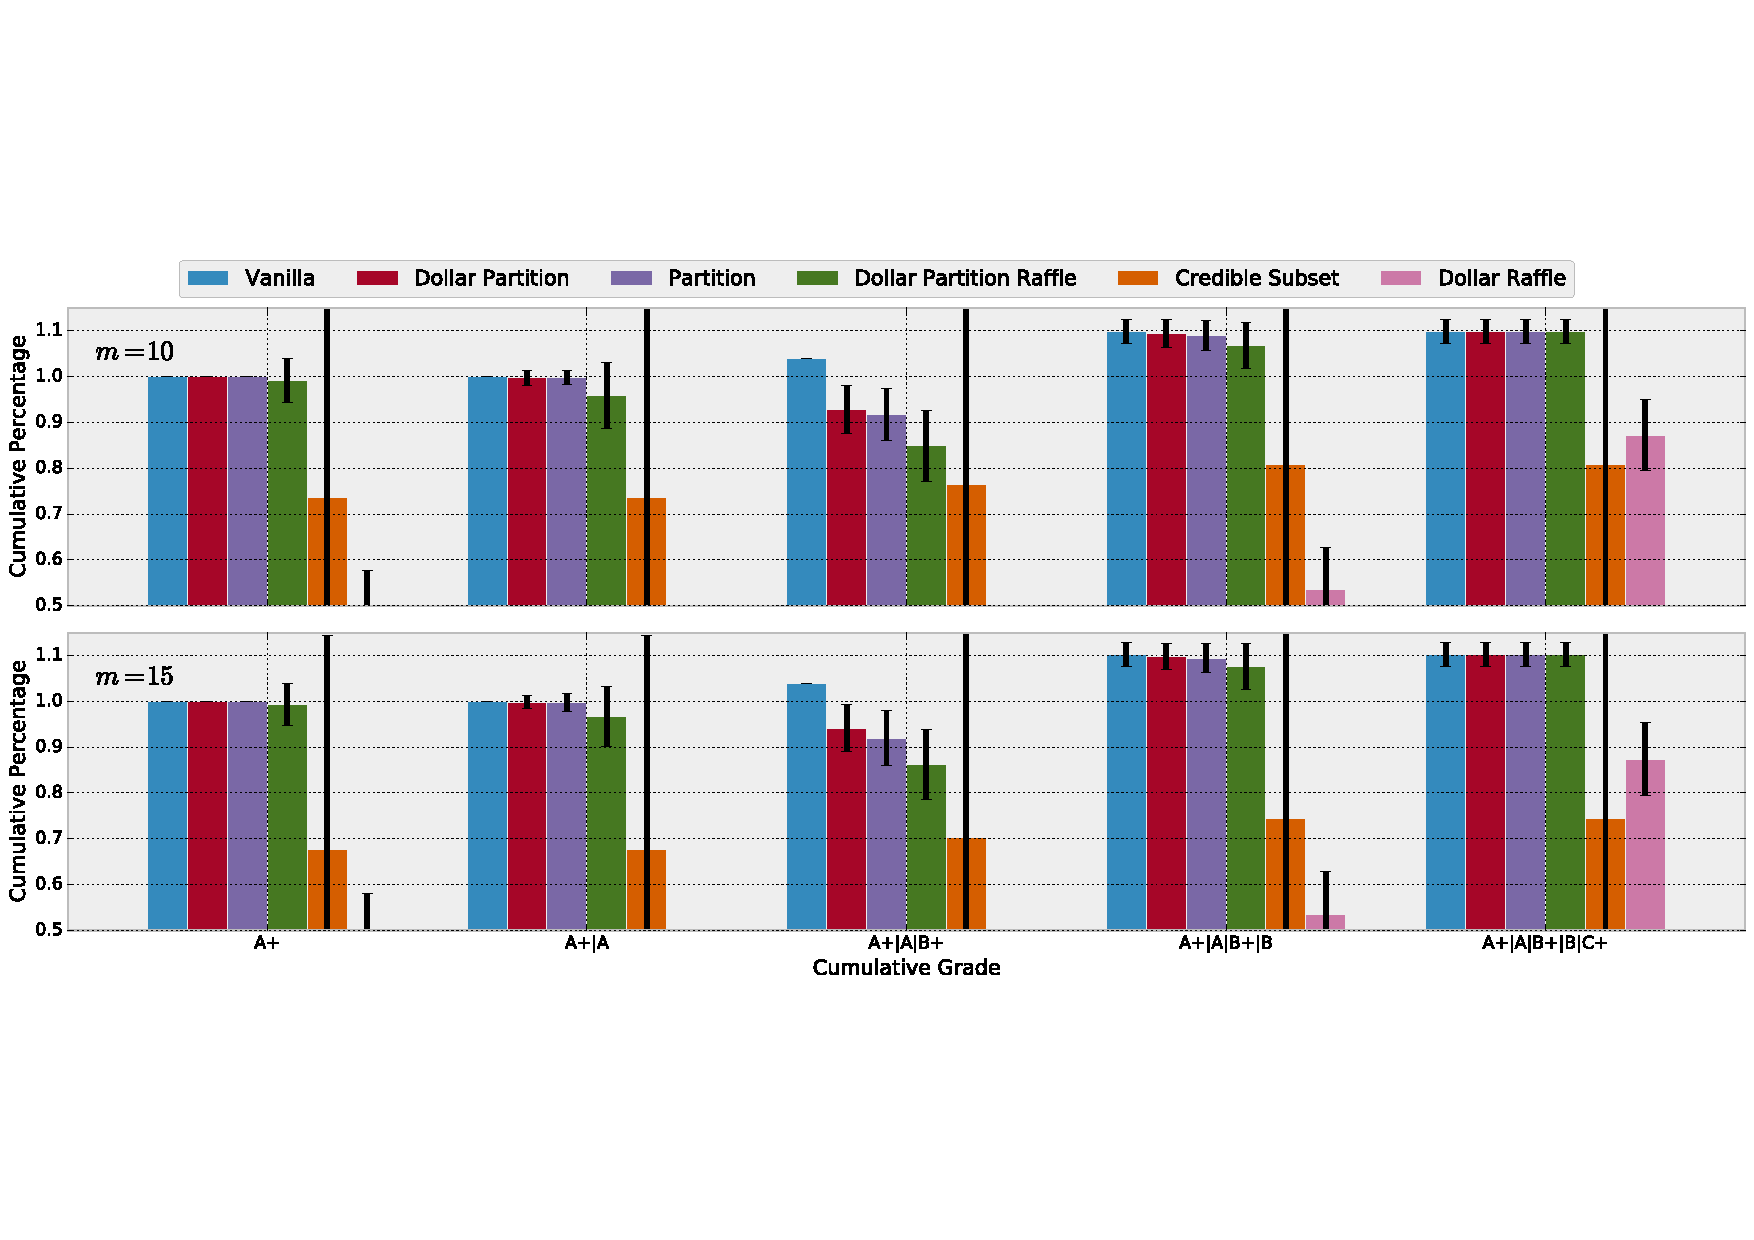
\includegraphics[width=.8\textwidth]{./cumulative_grade_big-emb}
\caption{Mean cumulative percentage of each grade of agent selected by the six peer selection algorithms presented in this paper on 1000 random iterations selecting $k=25$ agents from a population of $n=130$ agents providing $m=10$ (top) and $m=15$ (bottom) reviews divided into $l=5$ clusters with a Mallows dispersion $\phi = 0.1$. To enable comparisons, every mechanism selects $|W|$ equal to that of Dollar Partition; hence the $\geq 1.0$ averages as $k=25$ is the denominator. 
Error bars represent one standard deviation from the mean. 
Dollar Partition selects more agents from a higher grade more often, selects more agents from a higher grade in the worst case, and does so more consistently, than any other strategyproof mechanism. To highlight Partition and Dollar Partition we have cropped results where they are the same (cutting off Dollar Raffle).}\label{fig:results}
\end{figure*}
%\hfill

Figure~\ref{fig:results} shows the performance of the six mechanisms discussed on two different metrics as we vary the number of reviews received. We fixed $\phi=0.1$ for this testing as setting $\phi \in \{0.0, 0.1, 0.25, 0.4\}$ had no significant effect. The graphs show the mean cumulative proportion of the agents in each grade that are selected by each of the mechanisms over 1000 samples. For instance, the 1.0 score received by Vanilla for both A+ and A+$|$A for all settings of $m$ mean that Vanilla always selects the 11 highest scoring agents in the ground truth ranking ($\sigma$). We use cumulative selection with respect to the ground truth ordering.  This partial sum is well defined for each set of grades and clearly shows where a particular mechanism is over- or under-performing. Each mechanism was allowed to select a number of proposals equal to the number of agents returned by Dollar Partition per iteration, hence the average cumulative selection is $>1.0$. 
Whilst Vanilla is the best in our experiment, strictly dominating all other mechanisms, it is the only non-strategyproof mechanism. In practice, agents may not report truthfully with Vanilla and so it can perform much worse.
%Vanilla is the best according to our metric of cumulative agent selection, strictly dominating all other mechanisms (of course, it is the only non-strategyproof one...). 
The other generalizations of Dollar are strictly dominated by Dollar Partition; our more nuanced mechanism yields a better selection. 

Comparing Dollar Partition and Partition ($m=\{10,15\}$), both mechanisms select all of the A+ grade agents on every iteration. 
Partition selects only $9/11$, in the worst case, of the A+$|$A, while Dollar Partition selects $10/11$, an $11\%$ improvement.
Considering the A+$|$A$|$B+ agents, Partition only selects $17/26$, while Dollar Partition selects $20/26$, a $\geq 17\%$ performance increase.
Neither mechanism ever selects an agent with rank lower than C+; even in the worst case, both perform better than every other strategyproof mechanism in our study.\footnote{It is hard to directly compare results for Credible Subset due to the large probability of returning an empty set. This problem is not easily overcome; removing the ability to return an empty set means Credible Subset is no longer strategyproof. When Credible Subset does return a set, it slightly outperforms other mechanisms.} Standard deviation is also higher for Partition for all these cases, indicating Partition is much more likely to make mistakes and select agents from a lower grade over agents in a higher grade. Dollar Partition performs better than Partition in the worst case, and performs better on average. In a low information setting (i.e., $m\leq5$), Partition does perform slightly better on average than Dollar Partition. However, Dollar Partition shows a lower variance and better worst case performance across all settings to $m$, demonstrating its robustness to lopsided clusterings.

% There are many tradeoffs between parameters and the assumptions on the underlying distribution. In general, varying other parameters, such as $k$, $\ell$, $D$ and $F$ did not change the ranking of mechanisms shown here. However, increasing the number of clusters, improved Dollar Partition's performance in comparison to Partition's, which may stem from the increased chance that Partition will select the bottom candidates of a given cluster instead of better ranked candidates in a different cluster. Accordingly, as it generally selects the top candidates, Partition's performance improves when scoring rules are exponential in comparison to less extreme scoring rules, such as Borda. 

\smallskip
\noindent
\textbf{General Results:} We explored a realistic part of the large parameter space to investigate the mechanisms. The practical upshot, after running hundreds of thousands of instances, is that there are numerous tradeoffs that system designers must consider, critically depending on their target domain. In general, varying other parameters, such as $k$, $\ell$, $D$ and $F$ did not change the ranking of mechanisms shown here. However, increasing the number of clusters improved Dollar Partition's performance in comparison to Partition's, which may stem from the increased chance that Partition will select the bottom candidates of a given cluster instead of better ranked candidates in a different cluster. Accordingly, as it generally selects the top candidates, Partition's performance improves when scoring rules are exponential in comparison to less extreme scoring rules, such as Borda. 

Dollar Partition is much better when there is sufficient information, in terms of the number of reviews and the granularity of the grades, to have a chance of recovering the ground truth ordering. Settings like conferences with $n=2000$ papers and $m=5$ reviews split into 5--8 grades often have no clear cutoff between accept and reject; the grades contain too many items. In these cases all the mechanisms perform poorly, as selecting a set of winners is akin to randomly selecting agents from the set of possible winners. See, e.g., the NIPS experiment\footnote{http://blog.mrtz.org/2014/12/15/the-nips-experiment.html} and the recent paper on the limits of noisy rank aggregation using data from the KDD conference \cite{JoRa15a}. As the ratio of $m$ to $n$ grows, and the granularity of the grades increases, it becomes possible to recover the ground truth ranking, and Dollar Partition outperforms the other mechanisms.



%\smallskip
% \textbf{Other General Experimental Observations:}\;
%\paragraph{Other General Observations.}
%In addition to the testing detailed above we ran a number of tests varying the large parameter space to investigate the performance of the mechanisms. There are many tradeoffs between parameters and the assumptions on the underlying distribution.
%The practical upshot, after running hundreds of thousands of instances, is that there are 
%numerous tradeoffs that system designers must consider critically depending on their target domain.
%This is one reason we are releasing our code in an easy to use format.
%We mention some interesting trends that we will explore in future work. 
%
%\begin{inparaenum}[(i)]
%\item Dollar Partition strictly outperforms Dollar Partition Raffle which outperforms
%DollarRaffle in all tests, independent of the settings to $n, k, m, \ell, \phi, D,$ and $F$.
%
%\item Partition never seems to perform that poorly. This is likely due
%to the fact that running a lot of samples means we do not hit the degenerate 
%cases where Partition performs poorly all that often.
%
%\item Partition outperforms Dollar Partition, on average, when $m$ is very small ($n=130, m=5$). As
%$m$ increases relative to $n$ Dollar Partition overtakes the performance of Partition. In this sense Dollar Partition does more with the additional information it receives, making better selections. In contrast, raising $m$ increases the probability that Credible Subset will return the empty set.
%
%\item In general, adding more clusters improves the performance of Dollar Partition
%relative to Partition. This is likely due to the intuitive notion that Partition is making amongst the lower ranked elements in each cluster. The top few agents in every cluster it selects from are likely
%to be good (assuming we select more than one agent from each cluster). Only when
%taking the last $l$ or $2l$ agents is Partition more likely to make mistakes and Dollar Partition (with
%it's ability to reallocate some selections) does better.
%
%\item In general, it seems that Partition does better than Dollar Partition using exponential scoring 
%functions. When using scoring vectors closer to Borda, Dollar Partition performs better than Partition.
%
%\item The partition based mechanisms seem to be very sensitive to the
%score distribution.
%
%\item Unless the ratio of $m$ to $k$ is extremely tiny, i.e., $\leq \frac{1}{500}$ 
%Credible Subset returns an empty set with far too much frequency to be practically useful.
%
%\item We can use the ordering returned by Vanilla or the ground truth ranking -- these may not
%be the same due to how we choose an $m$-regular graph. For this reason we measure
%the quality of selection with respect to both the ground truth ordering and the Vanilla ordering as 
%this lets us compare to our true aim (the ground truth) as well as to the naive algorithm being implemented in some places \cite{KLMP15b}.
%
%\item Dollar Partition is much better when the agents can actually be compared -- when it is 
%not unreasonable to think there is a ground truth ordering that could be recovered. Working 
%with IJCAI like numbers of $2,000$ submissions and $m=5$ there is almost so little 
%information as to be a random process. See, e.g., the NIPS experiment\footnote{http://blog.mrtz.org/2014/12/15/the-nips-experiment.html}
%and the recent paper on the limits of noisy rank aggregation using data from the KDD conference \cite{JoRa15a}.
%Essentially, there are more than enough agents that receive high scores and the real challenge is pairing down into
%an acceptable size the subset of agents that are selected.
%\haris{How do we say what is a qualified paper? Do people do actual judging of whether a paper has enough quality or is just a non-jugmental ordinal feedback?} \nick{I will revise this -- realistically they just say that if you just use borda scores and a cutoff you end up with a lot of highly ranked papers, more than you can actually take... this is an intuitive argument that I will likely make more clear.}
%
%\item When comparing the other mechanisms against the the cumulative selection of the top-$k$ elements
%selected by Vanilla, Partition performs a bit better than Dollar Partition with respect to the individual elements.
%However, as our tests above showed, when we only look at the \emph{grades} selected, Dollar Partition
%performs better. This baseline gives us a notion of how close each of the mechanisms
%come to approximating the Vanilla \emph{ordering}; which can be seen as the best achievable given
%the noisy $m$-regular graph.
%\end{inparaenum}


%\subsection{Other General Experimental Observations}
%
%\begin{itemize}
%\item Partition never seems to perform that poorly. This is likely due
%to the fact that running a lot of samples means we do not hit the degenerate 
%cases where Partition performs poorly all that often.
%
%\item Dollar Partition is inherently \emph{nonjudgemental}. This is a nontechnical term which describes the following idea: since we normalize the scores outside the cluster in Dollar Partition we end up assigning the same scores to the ratings of agent $i$ who has a basket $m$ of all top proposals and agent $i'$ who has a basket $m'$ of all bottom proposals. We rely on an ordinal notion of comparisons
%with Dollar Partition; this ends up limiting how much one agent can affect the outcome.
%
%\item Partition outperforms Dollar Partition when $m$ is very small ($n=130, m=6$). As
%$m$ increases relative to $n$ Dollar Partition overtakes the performance of Partition. In this sense Dollar Partition does more with the additional information it receives, making better selections. In contrast raising $m$ increases the probability that Credible Subset will return the empty set. \nick{some slightly mushier argument against partition to go here.}
%
%\item In general, adding more clusters improves the performance of Dollar Partition
%relative to Partition. This is likely due to the intuitive notion that Partition is making mistakes
%at the bottom of its selection. The top few agents in every cluster it selects from are likely
%to be good (assuming we select more than one agent from each cluster). Only when
%taking the last $l$ or $2l$ agents is Partition more likely to make mistakes and Dollar Partition (with
%it's ability to reallocate some selections) does better.
%
%\haris{This is a request to please use partition accurately. We do not increase the number of partitions but the number of \emph{clusters in a partition}. This kind of usage is used in other places as well.}
%\omer{Think I fixed all such occurrences.}\haris{Thanks}
%
%\item In general, it seems that Partition does better than Dollar Partition using exponential scoring 
%functions. This is likely due to the nonjudgemental nature of Dollar Partition described above but 
%we are unsure.
%
%\item In settings where $m = n-1$ and a Borda like scoring vector Dollar Partition almost always
%out-preform all other mechanisms independent of $k$ or $l$.
%
%\item Dollar Partition strictly outperforms Dollar Partition Raffle which outperforms
%DollarRaffle in all tests, independent of the settings to $n, k, m, \ell, \phi, d,$ and $f$.
%
%\item The partition based mechanisms seem to be very sensitive to the
%score distribution.
%
%\item Unless the ratio of $m$ to $k$ is extremely tiny, i.e., $\leq \frac{1}{500}$ 
%Credible Subset returns an empty set with far too much frequency to be practically useful.
%A conference just ``not happening'' because the mechanism needs to be strategyproof
%does not seem realistic.
%
%\item We can use the ordering returned by Vanilla or the ground truth ranking -- these may not
%be the same due to how we choose an $m$-regular graph. For this reason we measure
%the quality of selection with respect to both the ground truth ordering and the Vanilla ordering as 
%this lets us compare to our true aim (the ground truth) as well as to the naive algorithm being implemented in some places \cite{KLMP15b}.
%
%\item Dollar Partition is much better when the agents can actually be compared -- when it is 
%not unreasonable to think there is a ground truth ordering that could be recovered. Working 
%with IJCAI like numbers of $2,000$ submissions and $m=5$ there is almost so little 
%information as to be a random process. See, e.g., the NIPS experiment\footnote{http://blog.mrtz.org/2014/12/15/the-nips-experiment.html}
%and the recent paper on the limits of noisy rank aggregation using data from the KDD conference \cite{JoRa15a}).
%Essentially, there are more than enough ``qualified'' papers and the real issue is pairing down into
%an acceptable size the subset of papers or proposals that could be reasonably selected.\haris{How do we say what is a qualified paper? Do people do actual judging of whether a paper has enough quality or is just a non-jugmental ordinal feedback?} \nick{I will revise this -- realistically they just say that if you just use borda scores and a cutoff you end up with a lot of highly ranked papers, more than you can actually take... this is an intuitive argument that I will likely make more clear.}
%
%\item There are too many tradeoffs between parameters to discuss at length here. 
%The practical upshot after running hundreds of thousands of settings is that there are 
%a lot of tradeoffs and system designers must think critically about what they want to achieve.
%This is one reason we are releasing our code in an easy to use format.
%
%\item We use the cumulative selection with respect the ground truth ordering because it 
%is well defined for each bin and the partial sum nature allows us to see where we are over 
%or underperforming.
%
%\item We also use the cumulative selection probability according to the top-$k$ elements
%selected by Vanilla. This result gives us an impression of how close each of the mechanisms
%come to approximating the Vanilla performance; which can be seen as the best achievable given
%the noisy $m$-regular graph.
%
%\item We ran with $\phi \in \{0.0, 0.1, 0.4\}$. The results seem to be the \emph{least} sensitive
%to this parameter. Therefore we stick with $\phi = 0.1$ in the experiment below.
%
%\end{itemize}


\section{Conclusion}
%This paper initiates a thorough comparison of different peer selection mechanisms, and introduces a new one -- Dollar Partition. This mechanism fares well in experiments, and though it has the drawback that it may return a few more agents than required, in practical settings it may not be a problem (for example, where a couple of more winners can be accommodated, or the award committee may have a shortlist that is slightly larger than the number of awardees, in case some agents are not able to take up the award offer). 

We introduce a novel peer selection mechanism---Dollar Partition.
Overall, Dollar Partition's flexibility in setting the number of agents to be selected from each cluster addresses the worst-case instances where partitions may be lopsided, allowing Dollar Partition to reach higher quality, more consistent results than existing mechanisms. Combined with the ability to always return a winning set, it is an improvement over current mechanisms.

%Though both Dollar Partition and the recently proposed Credible Subset are strategyproof, Dollar Partition not only performs better, but along with other Partition mechanisms, 
Among strategyproof mechanisms, Partition and Dollar Partition may 
have a certain `psychological' advantage: they may incentivize agents to report truthfully because an agent's contribution in selecting other agents (with whom he is not competing) is more direct.
%, and Dollar Partition also allows an inner ranking of its candidates. 
%In Credible Subset, however, all the potential winners are lumped together. 
Moreover, partitioning into groups helps deal with conflict of interest cases, when there is fear of collusion among several agents; putting them in the same cluster prevents them from influencing one another's chance of success.
Peer selection is a fundamental problem that has received less attention than voting rules.  We envisage the need to develop robust solutions with good incentive properties, as these are widely applicable in large-scale, crowdsourcing settings.

\section*{Acknowledgments}
Data61 (formerly known as NICTA) is funded by the Australian Government through the Department of Communications and the Australian Research Council through the ICT Centre of Excellence Program. This research has also been partly funded by Microsoft Research through its PhD Scholarship Program, and by Israel Science Foundation grant \#1227/12. This work has also been partly supported by COST Action IC1205 on Computational Social Choice.

\normalsize
\bibliographystyle{aaai}
\bibliography{abb,prizerefs}

%\begin{thebibliography}{}
%
%\bibitem[\protect\citeauthoryear{Alfaro and Shavlovsky}{2014}]{DeSh13a}
%Alfaro, L.~D., and Shavlovsky, M.
%\newblock 2014.
%\newblock {CrowdGrader: Crowdsourcing the Evaluation of Homework Assignments}.
%\newblock In {\em Proceedings of the ACM Technical Symposium on Computer
%  Science Education (ACM-SIGCSE)},  415--420.
%
%\bibitem[\protect\citeauthoryear{Alon \bgroup et al\mbox.\egroup
%  }{2011}]{AFPT11a}
%Alon, N.; Fischer, F.; Procaccia, A.~D.; and Tennenholtz, M.
%\newblock 2011.
%\newblock Sum of us: Strategyproof selection from the selectors.
%\newblock In {\em Proceedings of the 13th Conference on Theoretical Aspects of
%  Rationality and Knowledge (TARK)},  101--110.
%
%\bibitem[\protect\citeauthoryear{Berga and Gjorgjiev}{2014}]{BeGj14a}
%Berga, D., and Gjorgjiev, R.
%\newblock 2014.
%\newblock Impartial social rankings.
%\newblock Working paper.
%
%\bibitem[\protect\citeauthoryear{Bousquet, Norin, and Vetta}{2014}]{BNV14a}
%Bousquet, N.; Norin, S.; and Vetta, A.
%\newblock 2014.
%\newblock A near-optimal mechanism for impartial selection.
%\newblock In {\em Proceedings of the 10th International Workshop on Internet
%  and Network Economics (WINE)}, Lecture Notes in Computer Science (LNCS).
%
%\bibitem[\protect\citeauthoryear{de Clippel, Moulin, and
%  Tideman}{2008}]{CMT08a}
%de~Clippel, G.; Moulin, H.; and Tideman, N.
%\newblock 2008.
%\newblock Impartial division of a dollar.
%\newblock {\em Journal of Economic Theory} 139:176--191.
%
%\bibitem[\protect\citeauthoryear{Fischer and Klimm}{2014}]{FeKl14a}
%Fischer, F., and Klimm, M.
%\newblock 2014.
%\newblock Optimal impartial selection.
%\newblock In {\em Proceedings of the 15th ACM Conference on Economics and
%  Computation (ACM-EC)},  803--820.
%\newblock ACM Press.
%
%\bibitem[\protect\citeauthoryear{Hazelrigg}{2013}]{Haze13a}
%Hazelrigg, G.~A.
%\newblock 2013.
%\newblock {Dear Colleague Letter: Information to Principal Investigators (PIs)
%  Planning to Submit Proposals to the Sensors and Sensing Systems (SSS) Program
%  October 1, 2013, Deadline}.
%\newblock NSF Website, http://www.nsf.gov/pubs/2013/nsf13096/nsf13096.jsp.
%
%\bibitem[\protect\citeauthoryear{Holzman and Moulin}{2013}]{HoMo13a}
%Holzman, R., and Moulin, H.
%\newblock 2013.
%\newblock Impartial nominations for a prize.
%\newblock {\em Econometrica} 81(1):173--196.
%
%\bibitem[\protect\citeauthoryear{Joachims and Raman}{2015}]{JoRa15a}
%Joachims, T., and Raman, K.
%\newblock 2015.
%\newblock Bayesian ordinal aggregation of peer assessments: A case study on
%  {KDD} 2015.
%\newblock Technical report, Cornell University.
%
%\bibitem[\protect\citeauthoryear{Kulkarni \bgroup et al\mbox.\egroup
%  }{2013}]{KWLC13a}
%Kulkarni, C.; Wei, K.; Le, H.; and Chia, K.~D.
%\newblock 2013.
%\newblock Peer and self assessment in massive online classes.
%\newblock {\em ACM Transactions on Computer Human Interaction (TOCHI)}
%  20(6):1--31.
%
%\bibitem[\protect\citeauthoryear{Kurokawa \bgroup et al\mbox.\egroup
%  }{2015}]{KLMP15b}
%Kurokawa, D.; Lev, O.; Morgenstern, J.; and Procaccia, A.~D.
%\newblock 2015.
%\newblock Impartial peer review.
%\newblock In {\em Proceedings of the 23rd International Joint Conference on
%  Artificial Intelligence (IJCAI)}.
%\newblock AAAI Press.
%
%\bibitem[\protect\citeauthoryear{Lakhani, Garvin, and Lonstein}{2010}]{LGE10}
%Lakhani, K.~R.; Garvin, D.~A.; and Lonstein, E.
%\newblock 2010.
%\newblock Topcoder (a): Developing software through crowdsourcing.
%\newblock {\em Harvard Business Review}.
%
%\bibitem[\protect\citeauthoryear{Lu and Boutilier}{2011}]{LuBo11a}
%Lu, T., and Boutilier, C.
%\newblock 2011.
%\newblock Learning {M}allows models with pairwise preferences.
%\newblock In {\em Proceedings of the 28th International Conference on Machine
%  Learning (ICML)},  145--152.
%
%\bibitem[\protect\citeauthoryear{Mackenzie}{2015}]{Mack15a}
%Mackenzie, A.
%\newblock 2015.
%\newblock Symmetry and impartial lotteries.
%\newblock {\em Games and Economic Behavior}.
%
%\bibitem[\protect\citeauthoryear{Mallows}{1957}]{Mall57a}
%Mallows, C.
%\newblock 1957.
%\newblock Non-null ranking models.
%\newblock {\em Biometrika} 44(1):114--130.
%
%\bibitem[\protect\citeauthoryear{Mattei and Walsh}{2013}]{MaWa13a}
%Mattei, N., and Walsh, T.
%\newblock 2013.
%\newblock Preflib: {A} library for preferences.
%  \textsc{http://www.preflib.org}.
%\newblock In {\em Proceedings of the 3rd International Conference on
%  Algorithmic Decision Theory (ADT)},  259--270.
%
%\bibitem[\protect\citeauthoryear{Merrifield and Saari}{2009}]{MeSa09a}
%Merrifield, M.~R., and Saari, D.~G.
%\newblock 2009.
%\newblock Telescope time without tears: a distributed approach to peer review.
%\newblock {\em Astronomy \& Geophysics} 50(4):4--16.
%
%\bibitem[\protect\citeauthoryear{Mowbray and Gollmann}{2007}]{MG07}
%Mowbray, M., and Gollmann, D.
%\newblock 2007.
%\newblock Electing the doge of venice: Analysis of a 13th century protocol.
%\newblock In {\em Proceedings of the IEEE Symposium on Computer Security
%  Foundations},  295--310.
%
%\bibitem[\protect\citeauthoryear{Naghizadeh and Liu}{2013}]{NaLi13a}
%Naghizadeh, P., and Liu, M.
%\newblock 2013.
%\newblock Incentives, quality, and risks: A look into the {NSF} proposal review
%  pilot.
%\newblock {\em arXiv preprint arXiv:1307.6528}  1--10.
%
%\bibitem[\protect\citeauthoryear{Piech \bgroup et al\mbox.\egroup
%  }{2013}]{PHCD+13a}
%Piech, C.; Huang, J.; Chen, Z.; Do, C.; Ng, A.; and Koller, D.
%\newblock 2013.
%\newblock Tuned models of peer assessment in {MOOC}s.
%\newblock In {\em Proceedings of the 6th International Conference on
%  Educational Data Mining (EDM)},  153--160.
%
%\bibitem[\protect\citeauthoryear{Popova, Regenwetter, and
%  Mattei}{2013}]{PRM13a}
%Popova, A.; Regenwetter, M.; and Mattei, N.
%\newblock 2013.
%\newblock A behavioral perspective on social choice.
%\newblock {\em Annals of Mathematics and Artificial Intelligence}
%  68(1--3):135--160.
%
%\bibitem[\protect\citeauthoryear{Robinson}{2001}]{Robi01a}
%Robinson, R.
%\newblock 2001.
%\newblock Calibrated peer review an application to increase student reading and
%  writing skills.
%\newblock {\em The American Biology Teacher} 63(7):474--476.
%
%\bibitem[\protect\citeauthoryear{Roos, Rothe, and Scheuermann}{2011}]{RRS11a}
%Roos, M.; Rothe, J.; and Scheuermann, B.
%\newblock 2011.
%\newblock How to calibrate the scores of biased reviewers by quadratic
%  programming.
%\newblock In {\em Proceedings of the 25th AAAI Conference on Artificial
%  Intelligence (AAAI)},  255--260.
%
%\bibitem[\protect\citeauthoryear{Walsh}{2014}]{Wals14a}
%Walsh, T.
%\newblock 2014.
%\newblock The {PeerRank} method for peer assessment.
%\newblock In {\em Proceedings of the 21st European Conference on Artificial
%  Intelligence (ECAI)},  909--914.
%
%\bibitem[\protect\citeauthoryear{Wright, Thornton, and
%  Leyton-Brown}{2015}]{WTL15a}
%Wright, J.; Thornton, C.; and Leyton-Brown, K.
%\newblock 2015.
%\newblock {Mechanical TA}: {P}artially automated high-stakes peer grading.
%\newblock In {\em Proceedings of the ACM Technical Symposium on Computer
%  Science Education (ACM-SIGCSE)}.
%
%\bibitem[\protect\citeauthoryear{Young}{1994}]{Youn94a}
%Young, H.~P.
%\newblock 1994.
%\newblock {\em Equity: in Theory and Practice}.
%\newblock Princeton University Press.
%
%\end{thebibliography}
%

\end{document}

